\documentclass{beamer}
\usepackage{beamerthemeshadow}
\usepackage{graphicx}
\usepackage{color}
\usepackage[utf8]{inputenc}
\usepackage{hyperref}
\usepackage{caption}
\usepackage[flushleft]{threeparttable}
\usepackage{subfigure}
\definecolor{bluebell}{rgb}{0.64, 0.64, 0.82}
\setbeamercolor{structure}{fg=bluebell}
\captionsetup[figure]{labelformat=empty}
\captionsetup[table]{labelformat=empty}


\def\d{{\fontencoding{T1}\selectfont\dj}}
\def\D{{\fontencoding{T1}\selectfont\DJ}}


\title{Tehničko i naučno pisanje}
\subtitle{Da li veštačka inteligencija može da zameni ljudsko postojanje?}
\author{Isidora Jevremović \and Filip Erak\ \and Lea Kojičić \and Sara Gojaković}
\institute{Matematički fakultet\\Univerzitet u Beogradu}
\date{
	\footnotesize{Beograd, 2022.}	
}

\begin{document}
\begin{frame}
	\thispagestyle{empty}
	\titlepage
\end{frame}

\addtocounter{framenumber}{-1}

\begin{frame}[fragile]\frametitle{Literatura}
	\begin{itemize}
		\item Seminarski rad koji smo radili na ovu temu možete naći na sledećem linku:
		(\url{https://github.com/saragojakovic19/12_TNP2022/blob/main/12_JevremovicKojicicErakGojakovic.pdf})
	\end{itemize}
\end{frame}

\begin{frame}
	\frametitle{Pregled} % Table of contents slide, comment this block out to remove it
	\tableofcontents[] 
\end{frame}
\section{Da li veštačka inteligencija može da zameni ljudsko postojanje?}

\subsection{Uvod}

\begin{frame}[fragile]\frametitle{Uvod}
	\begin{itemize}	
		\item Rad Alana Tjuringa je bio uvod u moderan računarski svet i vizija pojma veštačke inteligencije.
		\item Pored svih prednosti koje veštačka inteligencija pruža postoje stvari u kojima ona ne može zameniti čoveka.
       \item Razlikujemo dve vrste veštačke inteligencije, jaku i slabu.
	\end{itemize}
 

 
\end{frame}

\subsection{Prirodna inteligencija}

\begin{frame}[fragile]\frametitle{Prirodna inteligencija}

        \begin{itemize}
        \item Antropocentrični način definisanja inteligencije.
        \item Najprihvaćenije definicije inteligencije su oprečne i značajno se razlikuju.
	\item Još jedan argument u korist ljudi je što nama tačna definicija nije ni potrebna, da bismo razumeli šta je sve inteligentno ponašanje.

        \begin{figure}[h!]
        \centering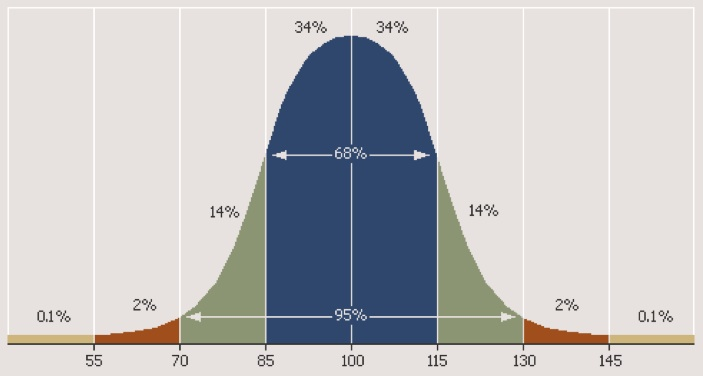
\includegraphics[height=3cm]{IQ.jpg}
        \caption{\emph{Gausova raspodela IQ testa}}
        \label{fig:raspodelaIQtesta}
    \end{figure}
\end{itemize}
\end{frame}

\begin{frame}[fragile]\frametitle{Klasifikacija na osnovu IQ testa}
\label{tab:tabelaIQ}
\begin{tabular}{|c|c|c|} \hline
IQ Domen & Klasifikacija & Procenat ljudske populacije\\ \hline
(55, 70]& Granična zaostalost & 2\%\\ \hline
(70, 85] & Zatupljenost & 14\%\\ \hline
(85, 115] & Prosečna inteligencija & 68\%\\ \hline
(115, 130] & Visok nivo inteligencije & 14\%\\ \hline
(130, 145] & Veoma visok nivo & 2\% \\ \hline
\end{tabular}

\end{frame}

\subsection{Veštačka inteligencija umesto čoveka}
\begin{frame}[fragile]\frametitle{Veštačka inteligencija umesto čoveka}
\begin{itemize}
    \item Veštačka inteligencija u saobraćaju
    \begin{itemize}
        \item Samovozeći automobili
        \item Autonomni brodovi
    \end{itemize}
    \item Veštačka inteligencija u okviru arheologije
    \begin{itemize}
        \item Ekspertni sistem PANDORA
    \end{itemize}
    \item Veštačka nauka u psihijatriji
    
\end{itemize}

\subsection{Zašto veštačka inteligencija ne može da zameni čoveka?}
\begin{frame}[fragile]\frametitle{Zašto veštačka inteligencija ne može da zameni čoveka?}

\begin{itemize}
    \item Uprkos svim ulaganjima, do sada je realizovana samo uska VI
    \item "Inteligentni" sistemi služe čoveku i oslanjaju se na njega u svom radu
    \item Proste radnje (poput prepoznavanja lica) zahtevaju mnogo novca, podataka, vremena i energije
\end{itemize}

\end{frame}

\section{Zaključak}

\begin{frame}[fragile]\frametitle{Zaključak}
        \begin{itemize}
            \item Moć inteligentnih sistema se ogleda u manipulaciji ogromnim količinama podataka i automatizaciji ljudskog ponašanja.
        \item Inteligencija sistema, u ljudskom smislu, je verovatno nemoguća.
        \item Glavna namena sistema VI je ušteda vremena, ne i potpuno preuzimanje odgovornosti za posao.
        \end{itemize}
\end{frame}

\end{frame}



\end{document}
